\chapter{Обзор предметной области}
\label{sec:domain}

В данном разделе будет произведён обзор предметной области задачи, решаемой в рамках диссертации; рассмотрены вопросы о сущности функционального и реактивного программирования и принципе их работы; также будут приведены существующие системы.

\section{Функциональное программирование}
\label{sub:domain:functional_programming}

Программы написанные на императивных языках программирования, таких как \csharp{}, \java{} или \cpp{}, в своей работе опираются на изменение значений набора переменных, называемого состоянием. Если мы пренебрежём операциями ввода-вывода и вероятностю того, что программы будет работать постоянно, то мы можем перейти к следующей абстракции. Первоначально состояние $\sigma$, представляющее собой входные данные для программы, а после завершения её исполнения --- новое значение $\sigma'$, представляющее результаты~\cite{intro2fp}. Выполнение отдельных операторов сводится к изменению ними состояния, которое последовательно проходит через конечное число значений:

\begin{equation}
  \label{eq:domain:states_transition}
  \sigma = \sigma_{0} \rightarrow \sigma_{1} \rightarrow \sigma_{2} \rightarrow ... \rightarrow \sigma_{n} = \sigma'
\end{equation}

Например, в программе сортировки состояние первоначально включает в себя массив значений, а после того, как программа завершается, состояние модифицируется таким образом, что эти значения становятся упорядоченными, в то время как промежуточные состояния представляют собой ход достижения данной цели.

Состояние обычно изменяется с помощью операторов присваивания, часто записываемых в виде $v = E$ или $v := E$, где $v$ --- переменная, а $E$ --- некоторое выражение. Последовательность выполнения таких операторов задаётся в тексте программы их размещением друг за другом (при этом часто в качестве разделителя применяется точка с запятой). С помощью составных операторов, таких как if и while, можно выполнять операторы в зависимости от условия или циклически, часто полагаясь на другие свойства текущего состояния. В результате программа превращается в набор инструкций по изменению состояния, и поэтому данный стиль программирования часто называется императивным или процедурным. Соответственно, традиционные языки программирования, поддерживающие такой стиль, также известны как императивные или процедурные языки.

Функциональное программирование радикально отличается от этой модели. По существу, функциональная программа представляет собой просто выражение, а выполнение программы процесс его вычисления. В общих чертах мы можем понять, как это возможно, используя следующие рассуждения. Предположим, что императивная программа (вся целиком) детерминирована, т.е. выход полностью определяется входом; мы можем сказать, что конечное состояние или тот его фрагмент, который нас интересует, являются функцией начального состояния, например $\sigma' = f(\sigma)$. В функциональном программировании эта точка зрения имеет особое значение: программа – это выражение, которое соответствует математической функции f. Функциональные языки поддерживают создание таких выражений за счет того, что позволяют использовать мощные функциональные конструкции~\cite{intro2fp}.

Функциональное программирование может противопоставляться императивному как c хорошей, так и в плохой стороны. К недостаткам ФП можно отнести то, что функциональные программы не используют переменные --- то есть не имеют состояния. Соответственно, они не могут использовать присваивание, поскольку нечему присваивать. Кроме того, идея последовательного выполнения операторов также бессмысленна, поскольку первый оператор не имеет никакого влияния на второй, так как нет никакого состояния, передаваемого между ними. К достоинствам функционального подхода можно отнести то, что функциональные программы могут использовать функции более изящным способом. Функции могут  рассматриваться	точно	так  же,  как  и  более	простые	объекты,  такие как целые числа: они	могут	передаваться в другие	функции	как аргументы и возвращаться в качестве результатов, а также применяться в вычислениях. Вместо последовательного выполнения операторов и использования циклов, функциональные языки программирования предлагают рекурсивные функции, т.е. функции, определённые в терминах самих себя. Большинство традиционных языков программирования обеспечивают весьма скудные возможности в этих областях. Язык C имеет некоторые ограниченные возможности работы с функциями при помощи указателей, но не позволяет создавать новые функции динамически. В языке \csharp{} существуют более широкие способы работы с функциями:

\begin{itemize}
  \item делегаты;
  \item лямбда-функции;
  \item анонимные типы;
\end{itemize}

На первый взгляд, язык без переменных или возможности последовательного выполнения инструкций кажется совершенно непрактичным. Многие свойства императивных языков программирования развились в процессе абстрагирования от типового компьютерного оборудования, от машинного кода к ассемблерам, затем к макроассемблерам, языку \cpp{} и так далее. Нет оснований утверждать, что такие языки представляют собой наиболее удобный способ взаимодействия человека и машины. В самом деле, последнее слово в развитии компьютерных архитектур еще не сказано, и компьютеры должны служить нашим нуждам, а не наоборот. Вероятно, что правильный подход не в том, чтобы начать с оборудования и продвигаться вверх, а наоборот – начать работу с языка программирования, как средства для описания алгоритмов, и затем двигаться вниз к оборудованию~\cite{dijkstra}. В действительности, данная тенденция может быть обнаружена и в традиционных языках программирования. Даже \cpp{} позволяет записывать арифметические выражения обычным способом. Программист не обеспокоен задачей линеаризации вычисления подвыражений и выделения памяти для хранения промежуточных результатов.

\section{Реактивное программирование}
\label{sub:domain:reactive_programming}

Реактивное программирование --- парадигма программирования, ориентированная на потоки данных и распространение изменений. Это означает, что должна существовать возможность легко выражать статические и динамические потоки данных, а также то, что нижележащая модель исполнения должна автоматически распространять изменения благодаря потоку данных.

К примеру, в императивном программировании присваивание $a := b + c$ будет означать, что переменной $a$ будет присвоен результат выполнения операции $b + c$, используя текущие (на момент вычисления) значения переменных. Позже значения переменных $b$ и $c$ могут быть изменены без какого-либо влияния на значение переменной $a$. В реактивном же программировании значение $a$ будет автоматически пересчитано, основываясь на новых значениях.

Системы построенные с помощью реактивного программирования обладают такими свойтвами~\ref{fig:reactive_scheme}:

\begin{itemize}
  \item событийно-ориентированость (Event-driven);
  \item масштабируемость (Scalable);
  \item отказоустойчивость (Resilient);
  \item отзывчивость (Responsive);
\end{itemize}

\begin{figure}[ht]
\centering
  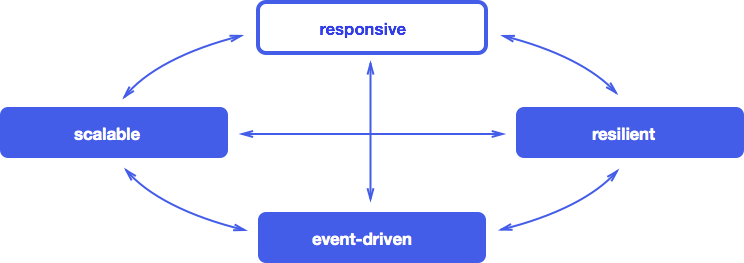
\includegraphics[scale=0.5]{reactive_scheme.png}
  \caption{ Принципы реактивного программирования }
  \label{fig:reactive_scheme}
\end{figure}

Это обеспечивает комфортное взаимодействие с пользователем, дающее ощущение реального времени и поддерживаемое самовосстанавливающимся масштабируемым прикладным стеком, готовым к развертыванию в многоядерных и облачных окружениях. Каждая из четырех характеристик реактивной архитектуры применяется ко всему технологическому стеку, что отличает их от звеньев в многоуровневых архитектурах. Рассмотрим их немного подробней.

\subsection{Event-driven. }
\label{subsub:domain:reactive_programming:event_driven}

Событийно-ориентированные приложения предполагают асинхронные коммуникации компонент и реализуют их слабую связанность (loosely coupled design): отправитель и получатель сообщения не нуждаются в сведениях ни друг о друге, ни о способе передачи сообщения, что позволяет им сконцентрироваться на содержании коммуникаций. Кроме того, что слабосвязанные компоненты значительно улучшают сопровождаемость, расширяемость и эволюционирование системы, асинхронность и неблокирующий характер их взаимодействия позволяют также освободить значительную часть ресурсов, снизить время оклика и обеспечить большую пропускную способность по сравнению с традиционными приложениями. Именно благодаря событийно-ориентированной природе возможны остальные черты реактивной архитектуры.

В событийно-ориентированном приложении компоненты взаимодействуют друг с другом путём отправки и получения сообщений --- дискретных частей информации, описывающих факты. Эти сообщения отправляются и принимаются в асинхронном и неблокирующем режиме. Модели построенные на событийно-ориентированной модели более склонны к push-модели, нежели чем к pull или poll. Т.е. они проталкивают данные к своим потребителям, когда данные становятся доступными, вместо того чтобы впустую тратить ресурсы, постоянно запрашивая или ожидая данные.

\begin{itemize}
  \item Асинхронная передача сообщений означает, что приложение по своей природе обладает высокой степенью конкуренции и может без изменений работать на многоядерной архитектуре. Любое ядро CPU может обработать любое сообщение, что даёт большие возможности параллелизации.
  \item Неблокирование означает способность продолжать работать, чтобы приложение было отзывчивым всё время, даже в условиях сбоя или пиковой нагрузки. Для этого все необходимые для обеспечения отзывчивости ресурсы, например CPU, память и сеть, не должно быть монополизированы. Это приведёт к более низкой латентности, большей пропускной способности и лучшей масштабируемости;
\end{itemize}

Традиционные серверные архитектуры используют общедоступное изменяемое состояние и блокирующие операции на одном потоке. Это вносит трудности при масштабировании системы. Общедоступное изменяемое состояние требует синхронизации, что привносит сложность и недетерменированность, делая код трудным для понимания и сопровождения. Переключение потока в спящий режим расходует ограниченные ресурсы, а пробуждение стоит дорого.

Разделяя генерацию событий и их обработку, мы позволяем платформе самой позаботиться о деталях синхронизации и диспетчеризации событий между потоками, в то время как мы сами концентрируемся на более высокоуровневых абстракциях и бизнес-логике. Мы думаем о том, откуда и куда пересылаются события, и о том, как компоненты взаимодействуют между собой, вместо того чтобы копаться с низкоуровневыми примитивами вроде потоков или блокировок.

Событийно-ориентированные модели обеспечивают слабую связанность между компонентами и подсистемами. Такая связанность, как мы увидим позже, является одним из необходимых условий масштабируемости и отказоустойчивости. Без сложных и сильных зависимостей между компонентами расширение системы требует минимальных усилий.

Когда от приложения требуется высокая производительность и хорошая масштабируемость, трудно предусмотреть, где могут возникнуть узкие места. Поэтому очень важно, чтобы всё решение было асинхронным и неблокирующим. Для типичного приложения это означает, что архитектура должна быть полностью событийно-ориентированной, начиная с запросов пользователей через графический интерфейс и обработки запросов в веб-слое и заканчивая сервисами, кэшем и базой данных. Если хотя бы один из этих слоёв не будет отвечать этому требованию --- будет делать блокирующие запросы в БД, использовать общедоступное изменяемое состояние, вызывать дорогие синхронные операции --- то весь стек заглохнет и пользователи будут страдать из-за возросших задержек и упавшей масштабируемости.

\subsection{Scalable. }
\label{subsub:domain:reactive_programming:scalable}

Масштабируемость в контексте реактивного программирования --- это реакция системы на изменение нагрузки, т.е. эластичность, достигаемая возможностью добавления или освобождения вычислительных узлов по мере необходимости. Благодаря низкой связанности, асинхронному обмену сообщениями и независимости от размещения компонент (location transparency), способ развертывания и топология приложения становятся решением времени развертывания и предметом конфигурации и адаптивных алгоритмов, реагирующих на нагрузку. Таким образом, вычислительная сеть становится частью приложения, изначально имеющего явную распределенную природу.

Событийно-ориентированная система, базирующаяся на асинхронной передаче сообщений, является основой масштабируемости. Слабая связанность и локационная независимость компонентов и подсистем позволяют разворачивать систему на множестве узлов, оставаясь в пределах той же самой программной модели с той же семантикой. При добавлении новых узлов возрастает пропускная способность системы. В терминах реализации не должно быть никакой разницы между развертыванием системы на большем количестве ядер или большем количестве узлов кластера или центра обработки данных. Топология приложения становится проблемой конфигурации и/или адаптивных алгоритмов времени выполнения, следящих за нагрузкой на систему. Это то, что мы называем локационной прозрачностью~\cite{location_transparency}.

Важно понимать, что цель --- не изобрести прозрачные распределённые вычисления, распределённые объекты или RPC-коммуникации --- это уже пытались сделать раньше и эта затея провалилась. Вместо этого мы должны охватить сеть, представив её прямым образом в программной модели через механизм асинхронных сообщений. Настоящая масштабируемость естественным образом полагается на распределённые вычисления и их межузловое взаимодействие, что означает обход сети, который по своей сути является ненадёжным. Поэтому важно учесть ограничения, компромиссы и сценарии исключительных ситуаций явно в программной модели вместо того, чтобы прятать их за ширмой дырявых абстракций, которые якобы пытаются «упростить» вещи. Как следствие, в равной степени важно обеспечить себя программными инструментами, содержащими в себе строительные блоки для решения типичных проблем, которые могут возникнуть в распределённом окружении --- вроде механизмов для достижения консенсуса или интерфейсов обмена сообщениями, которые обладают высоким уровнем надёжности.

\subsection{Resilent. }
\label{subsub:domain:reactive_programming:resilent}

Отказоустойчивость реактивной архитектуры тоже становится частью дизайна, и это значительно отличает ее от традиционных подходов к обеспечению непрерывной доступности системы путем резервирования серверов и перехвата управления при отказе. Устойчивость такой системы достигается ее способностью корректно реагировать на сбои отдельных компонент, изолировать эти сбои, сохраняя их контекст в виде вызвавших их сообщений, и передавать эти сообщения другому компоненту, способному принять решения о том, как следует обрабатывать ошибку. Такой подход позволяет сохранить чистой бизнес-логику приложения, отделив от нее логику обработки сбоев, которая формулируется в явном декларативном виде для регистрации, изолирования, и обработки сбоев средствами самой системы. Для построения таких самовосстанавливающихся систем компоненты упорядочиваются иерархически, и проблема эскалируется до того уровня, который способен ее решить.

Чтобы управлять сбоями, нам нужен способ изолировать их, так чтобы они не распространялись на другие работоспособные компоненты, и вести за ними наблюдение из безопасного места вне контекста, в котором могут происходить сбои. Один способ, который приходит на ум, --- это переборки, разделяющие систему на отсеки таким образом, что если затапливается один из отсеков (выходит из строя), то это никак не влияет на другие отсеки. Это предотвращает классическую проблему каскадных сбоев и позволяет решать проблемы изолированно.

Событийно-ориентированная модель, которая даёт масштабируемость, также предоставляет необходимые примитивы для решения проблемы отказоустойчивости. Слабая связанность в событийно-ориентированной модели снабжает нас полностью изолированными компонентами, в которых сбои инкапсулируются в сообщения вместе с необходимыми деталями и пересылаются другим компонентам, которые в свою очередь анализируют ошибки и решают, как реагировать на них.

Такой подход создаёт систему, в которой:

\begin{itemize}
  \item бизнес-логика остаётся чистой, отделённой от обработки ошибок;
  \item сбои моделируются явно, чтобы разбиение на отсеки, наблюдение, управление и конфигурация задавались декларативно;
  \item система может «лечить» себя и восстанавливаться автоматически;
\end{itemize}

Лучше всего, если отсеки организуются иерархическим образом, подобно большой корпорации, где проблемы поднимаются до уровня, имеющего достаточно власти, чтобы принять соответствующие меры.

Мощь данной модели в том, что она чисто событийно-ориентированная --- она основана на реактивных компонентах и асинхронных событиях, и поэтому обладает локационной прозрачностью. На практике это означает, что её семантика не зависит от того, работает ли она на локальном сервере или в распределённом окружении.

\subsection{Responsive. }
\label{subsub:domain:reactive_programming:responsive}

И наконец отзывчивость --- это способность системы реагировать на пользовательское воздействие независимо от нагрузки и сбоев, такие приложения вовлекают пользователя во взаимодействие, создают ощущение тесной связи с системой и достаточной оснащенности для выполнения текущих задач. Отзывчивость актуальна не только в системах реального времени, но и необходима для широкого круга приложений. Более того, система, неспособная к быстрому отклику даже в момент сбоя, не может считаться отказоустойчивой. Отзывчивость достигается применением наблюдаемых моделей (observable models), потоков событий (event streams) и клиентов с состоянием (stateful clients). Наблюдаемые модели генерируют события при изменении своего состояния и обеспечивают взаимодействие реального времени между пользователями и системами, а потоки событий предоставляют абстракцию, на которой построено это взаимодействие путем неблокирующих асинхронных трансформаций и коммуникаций.

Реактивные приложения используют наблюдаемые модели, потоки событий и клиенты с состоянием.

Наблюдаемые модели позволяют другим системам получать события, когда их состояние изменяется. Это обеспечивает связь в реальном времени между пользователями и системами. Например, когда несколько пользователей работают одновременно над одной и той же моделью, изменения могут реактивно синхронизироваться между ними, избавляя от необходимости блокировки модели.

Потоки событий образуют базовую абстракцию, на которой строятся такие связи. Сохраняя их реактивными, мы избегаем блокировок и позволяем преобразованиям и коммуникациям быть асинхронными и неблокирующими.

Реактивные приложения должны иметь понятие о порядках алгоритмов~\cite{algh_complexity}, чтобы быть уверенным, что время отклика на события не превышает O(1) или, как минимум, O(log n) независимо от нагрузки. Может быть включён коэффициент масштабирования, но он не должен зависеть от количества клиентов, сессий, продуктов или сделок.

Вот несколько стратегий, которые помогут сохранить латентность независимой от профиля нагрузки:

\begin{itemize}
  \item В случае взрывного трафика реактивные приложения должны амортизировать затраты на дорогие операции, такие как ввод-вывод или конкурентный обмен данными, применяя batching с пониманием и учитыванием специфики низлежащих ресурсов.
  \item Очереди должны быть ограничены с учётом интенсивности потока, длины очередей при данных требованиях на время отклика должны определяться согласно закону Литтла~\cite{little_law}.
  \item Системы должны находиться в состоянии постоянного мониторинга и иметь адекватный запас прочности.
  \item В случае сбоев активируются автоматические выключатели и запускаются запасные стратегии обработки~\cite{circuit_breaker_design_pattern}.
\end{itemize}

В качестве примера рассмотрим отзывчивое веб-приложение с «богатыми» клиентами (браузер, мобильное приложение), чтобы предоставить пользователю качественный опыт взаимодействия. Это приложение исполняет логику и хранит состояние на стороне клиента, в котором наблюдаемые модели предоставляют механизм обновления пользовательского интерфейса при изменении данных в реальном времени. Технологии вроде WebSockets или Server-Sent Events позволяют пользовательскому интерфейсу соединяться напрямую с потоком событий, так что система целиком становится событийно-ориентированной, начиная с back-end слоя и заканчивая клиентом. Это позволяет реактивным приложениям проталкивать события браузеру и мобильным приложениям посредством асинхронной и неблокирующей передачи данных, сохраняя масштабируемость и отказоустойчивость.

Таким образом, реактивные приложения представляют собой сбалансированный подход к решению широкого спектра задач современной разработки ПО. Построенные на событийно-ориентированном основании, они предоставляют средства, необходимые для гарантий масштабируемости и отказоустойчивости и поддерживают полнофункциональное отзывчивое пользовательское взаимодействие~\cite{reactive_manifesto}.
